\documentclass[11pt,a4paper]{report}
\usepackage[textwidth=37em,vmargin=30mm]{geometry}
\usepackage{calc,xunicode,amsmath,amssymb,paralist,enumitem,tabu,booktabs,datetime2,xeCJK,xeCJKfntef,listings}
\usepackage{tocloft,fancyhdr,tcolorbox,xcolor,graphicx,eso-pic,xltxtra,xelatexemoji}

\newcommand{\envyear}[0]{2025}
\newcommand{\envdatestr}[0]{2025-06-29}
\newcommand{\envfinaldir}[0]{webdb/2025/20250629/final}

\usepackage[hidelinks]{hyperref}
\hypersetup{
    colorlinks=false,
    pdfpagemode=FullScreen,
    pdftitle={Web Digest - \envdatestr}
}

\setlength{\cftbeforechapskip}{10pt}
\renewcommand{\cftchapfont}{\rmfamily\bfseries\large\raggedright}
\setlength{\cftbeforesecskip}{2pt}
\renewcommand{\cftsecfont}{\sffamily\small\raggedright}

\setdefaultleftmargin{2em}{2em}{1em}{1em}{1em}{1em}

\usepackage{xeCJK,xeCJKfntef}
\xeCJKsetup{PunctStyle=plain,RubberPunctSkip=false,CJKglue=\strut\hskip 0pt plus 0.1em minus 0.05em,CJKecglue=\strut\hskip 0.22em plus 0.2em}
\XeTeXlinebreaklocale "zh"
\XeTeXlinebreakskip = 0pt


\setmainfont{Brygada 1918}
\setromanfont{Brygada 1918}
\setsansfont{IBM Plex Sans}
\setmonofont{JetBrains Mono NL}
\setCJKmainfont{Noto Serif CJK SC}
\setCJKromanfont{Noto Serif CJK SC}
\setCJKsansfont{Noto Sans CJK SC}
\setCJKmonofont{Noto Sans CJK SC}

\setlength{\parindent}{0pt}
\setlength{\parskip}{8pt}
\linespread{1.15}

\lstset{
	basicstyle=\ttfamily\footnotesize,
	numbersep=5pt,
	backgroundcolor=\color{black!5},
	showspaces=false,
	showstringspaces=false,
	showtabs=false,
	tabsize=2,
	captionpos=b,
	breaklines=true,
	breakatwhitespace=true,
	breakautoindent=true,
	linewidth=\textwidth
}






\newcommand{\coverpic}[2]{
    % argv: itemurl, authorname
    Cover photo by #2~~(\href{#1}{#1})
}
\newcommand{\makeheader}[0]{
    \begin{titlepage}
        % \newgeometry{hmargin=15mm,tmargin=21mm,bmargin=12mm}
        \begin{center}
            
            \rmfamily\scshape
            \fontspec{BaskervilleF}
            \fontspec{Old Standard}
            \fontsize{59pt}{70pt}\selectfont
            WEB\hfill DIGEST
            
            \vfill
            % \vskip 30pt
            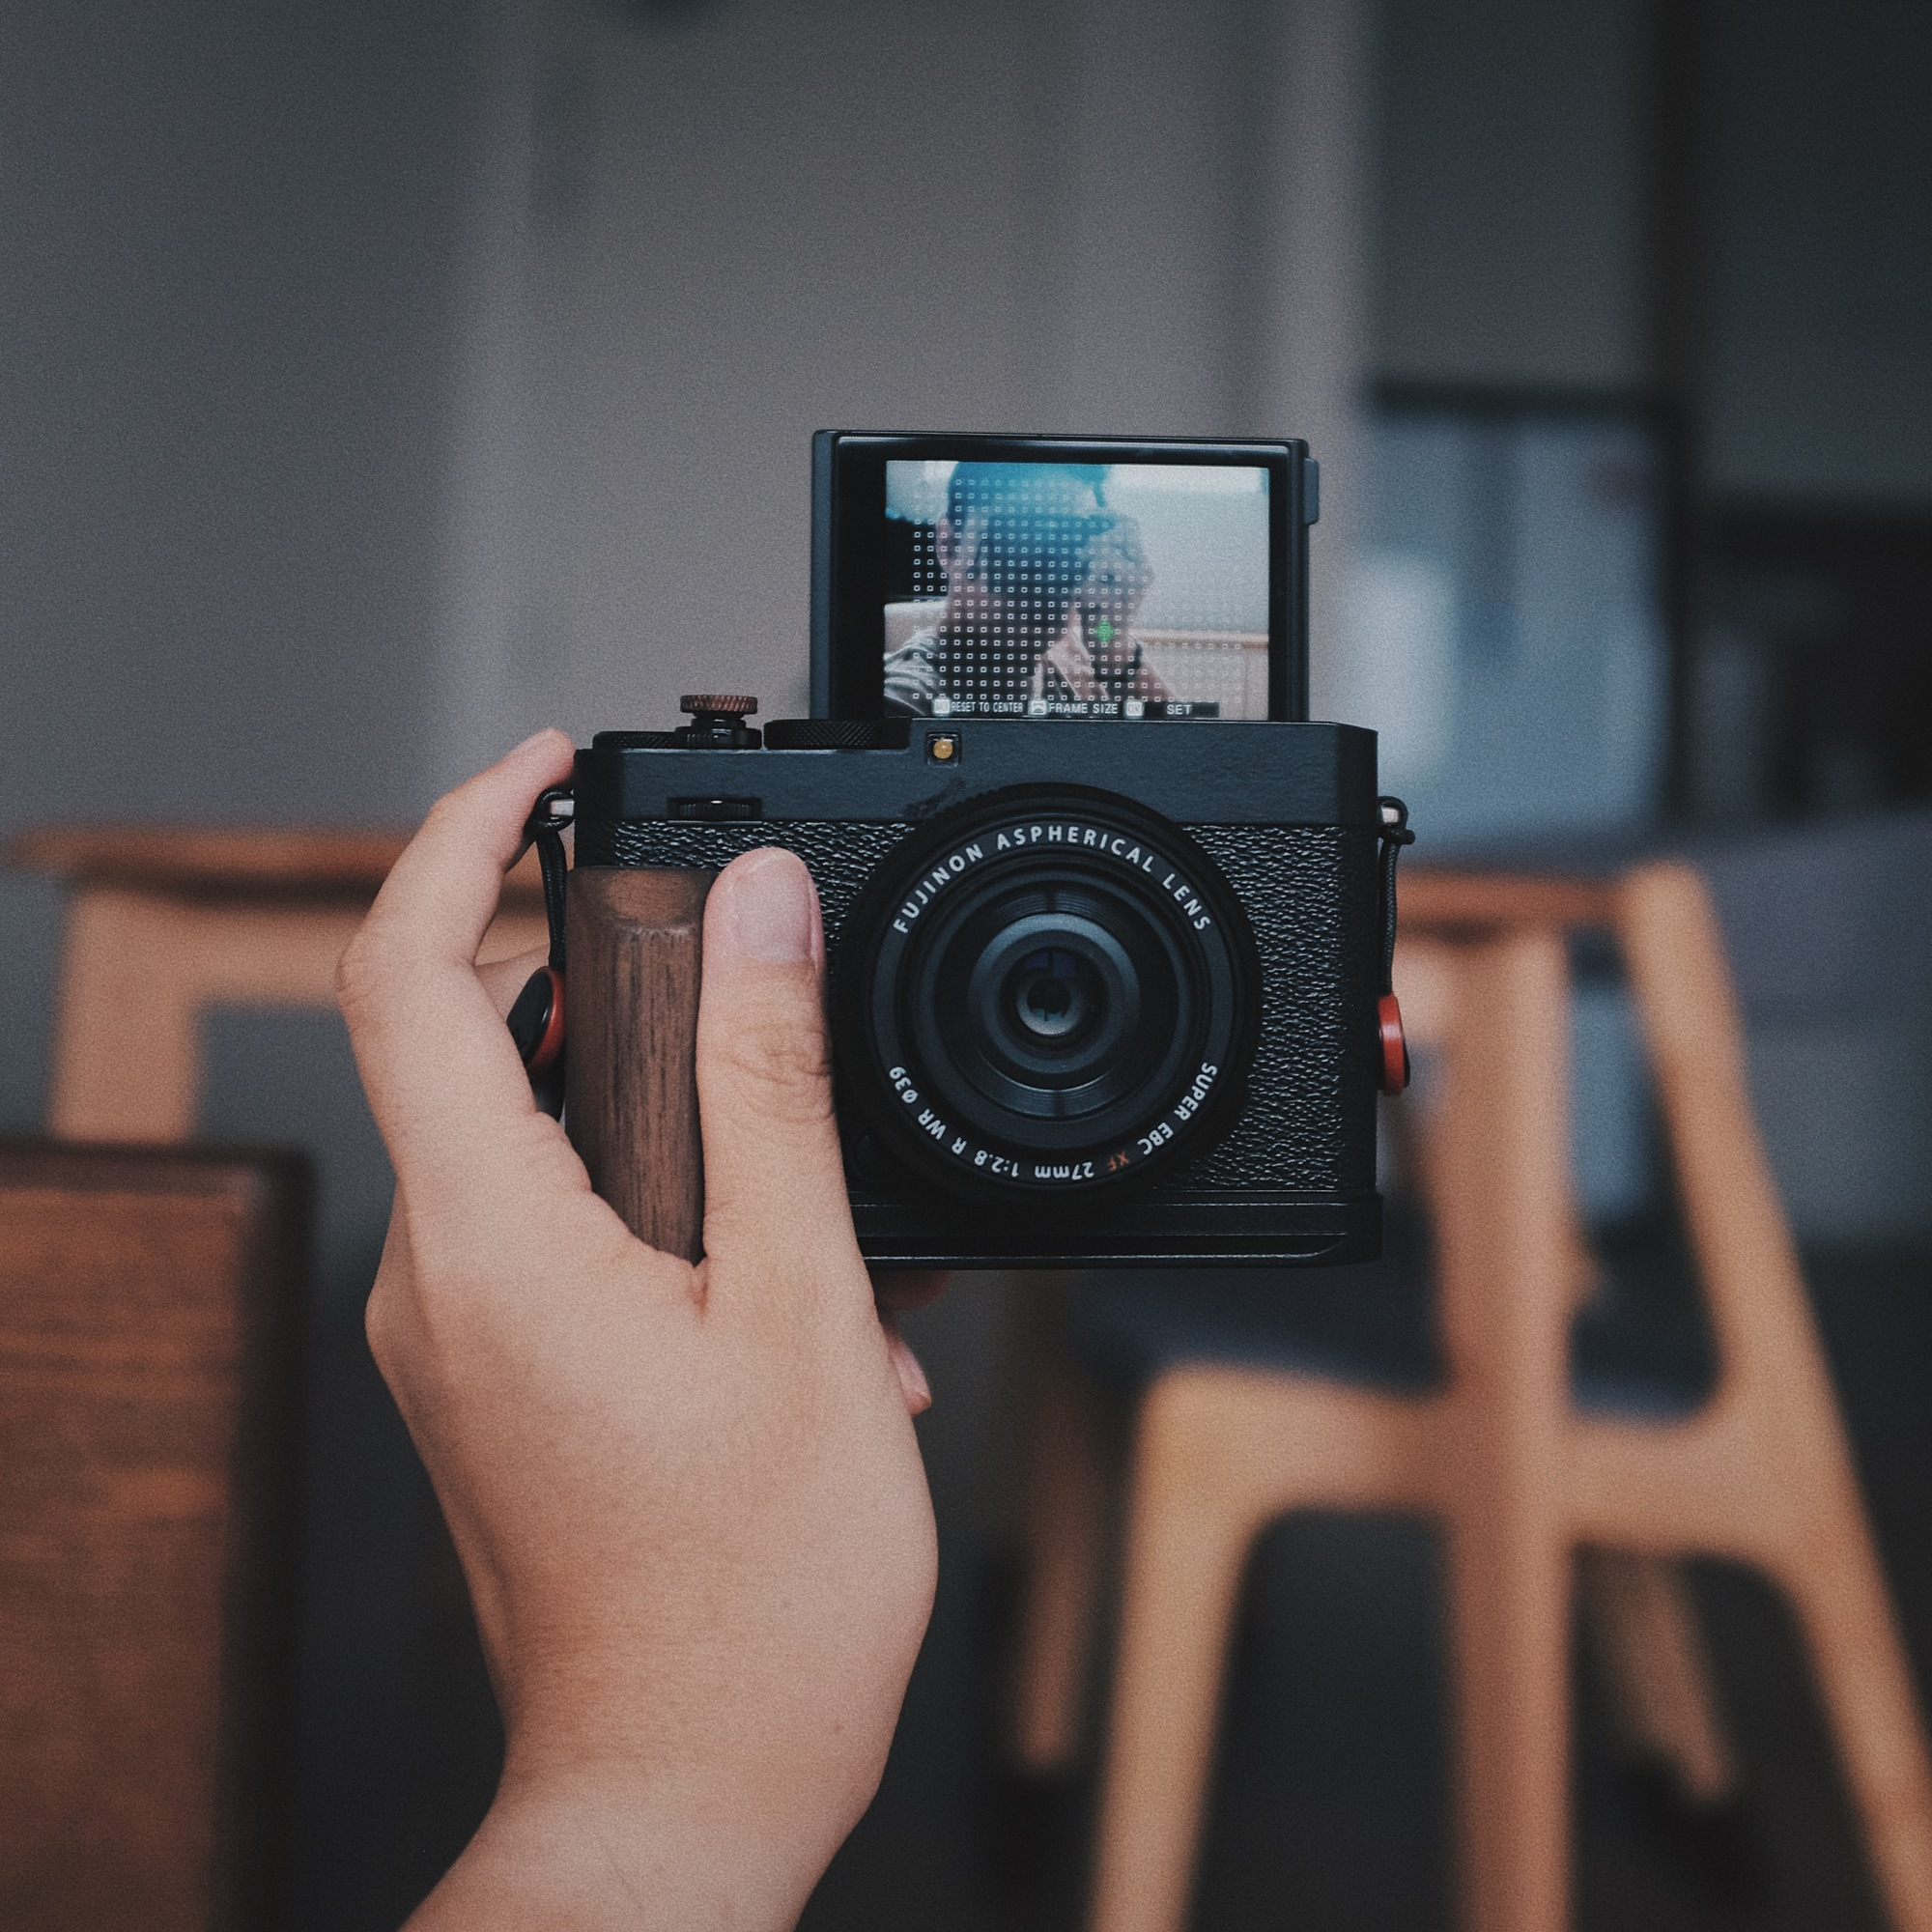
\includegraphics[width=\linewidth]{\envfinaldir/coverpic-prod.jpg}\par
            % \vskip 30pt
            \vfill

            \normalsize\rmfamily\scshape
            \copyright{} The Web Digest Project \hfill\large \envdatestr
        \end{center}
    \end{titlepage}
    % \restoregeometry
}
\newcommand{\simplehref}[1]{%
    \textcolor{blue!80!green}{\href{#1}{#1}}%
}
\renewcommand{\contentsname}{\center\Huge\sffamily\bfseries Contents\par\vskip 20pt}
\newcounter{ipartcounter}
\setcounter{ipartcounter}{0}
\newcommand{\ipart}[1]{
    % \vskip 20pt
    \clearpage
    \stepcounter{ipartcounter}
    \phantomsection
    \addcontentsline{toc}{chapter}{#1}
    % \begin{center}
    %     \Huge
    %     \sffamily\bfseries
    %     #1
    % \end{center}
    % \vskip 20pt plus 7pt
}
\newcounter{ichaptercounter}
\setcounter{ichaptercounter}{0}
\newcommand{\ichapter}[1]{
    % \vskip 20pt
    \clearpage
    \stepcounter{ichaptercounter}
    \phantomsection
    \addcontentsline{toc}{section}{\numberline{\arabic{ichaptercounter}}#1}
    \begin{center}
        \Huge
        \sffamily\bfseries
        #1
    \end{center}
    \vskip 20pt plus 7pt
}
\newcommand{\entrytitlefont}[1]{\subsection*{\raggedright\Large\sffamily\bfseries#1}}
\newcommand{\entryitemGeneric}[2]{
    % argv: title, url
    \parbox{\linewidth}{
        \entrytitlefont{#1}\par\vskip 5pt
        \footnotesize\ttfamily\mdseries
        \simplehref{#2}
    }\vskip 11pt plus 11pt minus 1pt
}
\newcommand{\entryitemGithub}[3]{
    % argv: title, url, desc
    \parbox{\linewidth}{
        \entrytitlefont{#1}\par\vskip 5pt
        \footnotesize\ttfamily\mdseries
        \simplehref{#2}\par\vskip 5pt
        \small\rmfamily\mdseries#3
    }\vskip 11pt plus 11pt minus 1pt
}
\newcommand{\entryitemAp}[3]{
    % argv: title, url, desc
    \parbox{\linewidth}{
        \entrytitlefont{#1}\par\vskip 5pt
        \footnotesize\ttfamily\mdseries
        \simplehref{#2}\par\vskip 5pt
        \small\rmfamily\mdseries#3
    }\vskip 11pt plus 11pt minus 1pt
}
\newcommand{\entryitemHackernews}[3]{
    % argv: title, hnurl, rawurl
    % \parbox{\linewidth}{
    %     \entrytitlefont{#1}\par\vskip 5pt
    %     \footnotesize\ttfamily\mdseries
    %     \simplehref{#3}\par
    %     \textcolor{black!50}{\href{#2}{#2}}
    % }\vskip 11pt plus 11pt minus 1pt
    \begin{minipage}{\linewidth}
            \entrytitlefont{#1}\par\vskip 5pt
            \footnotesize\ttfamily\mdseries
            \simplehref{#3}\par
            \textcolor{black!50}{\href{#2}{#2}}
    \end{minipage}\par\vskip 11pt plus 11pt minus 1pt
}







\begin{document}

\makeheader

\tableofcontents\clearpage




\ipart{Developers}
\ichapter{Hacker News}
\entryitemTwoLinks{JavaScript Trademark Update}{https://news.ycombinator.com/item?id=44407139}{https://deno.com/blog/deno-v-oracle4}

\entryitemTwoLinks{No One Is in Charge at the US Copyright Office}{https://news.ycombinator.com/item?id=44406400}{https://www.wired.com/story/us-copyright-office-chaos-doge/}

\entryitemTwoLinks{BusyBeaver(6) Is Quite Large}{https://news.ycombinator.com/item?id=44406171}{https://scottaaronson.blog/?p=8972}

\entryitemTwoLinks{Addictions Are Being Engineered}{https://news.ycombinator.com/item?id=44405057}{https://masonyarbrough.substack.com/p/engineered-addictions}

\entryitemTwoLinks{MCP: An (Accidentally) Universal Plugin System}{https://news.ycombinator.com/item?id=44404905}{https://worksonmymachine.substack.com/p/mcp-an-accidentally-universal-plugin}

\entryitemTwoLinks{We ran a Unix-like OS Xv6 on our home-built CPU with a home-built C compiler (2020)}{https://news.ycombinator.com/item?id=44404164}{https://fuel.edby.coffee/posts/how-we-ported-xv6-os-to-a-home-built-cpu-with-a-home-built-c-compiler/}

\entryitemTwoLinks{Unheard works by Erik Satie to premiere 100 years after his death}{https://news.ycombinator.com/item?id=44403594}{https://www.theguardian.com/music/2025/jun/26/unheard-works-by-erik-satie-to-premiere-100-years-after-his-death}

\entryitemTwoLinks{IDF officers ordered to fire at unarmed crowds near Gaza food distribution sites}{https://news.ycombinator.com/item?id=44402896}{https://www.haaretz.com/israel-news/2025-06-27/ty-article-magazine/.premium/idf-soldiers-ordered-to-shoot-deliberately-at-unarmed-gazans-waiting-for-humanitarian-aid/00000197-ad8e-de01-a39f-ffbe33780000}

\entryitemTwoLinks{I deleted my second brain}{https://news.ycombinator.com/item?id=44402470}{https://www.joanwestenberg.com/p/i-deleted-my-second-brain}

\entryitemTwoLinks{Facebook is asking to use Meta AI on photos you haven't yet shared}{https://news.ycombinator.com/item?id=44401406}{https://www.theverge.com/meta/694685/meta-ai-camera-roll}

\entryitemTwoLinks{Rust in the Linux kernel: part 2}{https://news.ycombinator.com/item?id=44400697}{https://lwn.net/SubscriberLink/1025232/fbb2d90d084368e3/}

\entryitemTwoLinks{Normalizing Flows Are Capable Generative Models}{https://news.ycombinator.com/item?id=44400105}{https://machinelearning.apple.com/research/normalizing-flows}

\entryitemTwoLinks{Learn OCaml}{https://news.ycombinator.com/item?id=44400025}{https://ocaml-sf.org/learn-ocaml-public/\#activity=exercises}

\entryitemTwoLinks{A brief history of children sent through the mail (2016)}{https://news.ycombinator.com/item?id=44399854}{https://www.smithsonianmag.com/smart-news/brief-history-children-sent-through-mail-180959372/}

\entryitemTwoLinks{SymbolicAI: A neuro-symbolic perspective on LLMs}{https://news.ycombinator.com/item?id=44399234}{https://github.com/ExtensityAI/symbolicai}

\entryitemTwoLinks{JWST reveals its first direct image discovery of an exoplanet}{https://news.ycombinator.com/item?id=44398756}{https://www.smithsonianmag.com/smart-news/james-webb-space-telescope-reveals-its-first-direct-image-discovery-of-an-exoplanet-180986886/}

\entryitemTwoLinks{US Supreme Court limits federal judges' power to block Trump orders}{https://news.ycombinator.com/item?id=44398710}{https://www.theguardian.com/us-news/2025/jun/27/trump-supreme-court-birthright-citizenship-scotus}

\entryitemTwoLinks{Transmitting data via ultrasound without any special equipment}{https://news.ycombinator.com/item?id=44398390}{https://halcy.de/blog/2025/06/27/transmitting-data-via-ultrasound-without-any-special-equipment/}

\entryitemTwoLinks{Project Vend: Can Claude run a small shop? (And why does that matter?)}{https://news.ycombinator.com/item?id=44397923}{https://www.anthropic.com/research/project-vend-1}

\entryitemTwoLinks{Weird Expressions in Rust}{https://news.ycombinator.com/item?id=44397367}{https://www.wakunguma.com/blog/rust-weird-expr}


\ipart{Developers~~~~(zh-Hans)}
\ichapter{Solidot}
\entryitemGeneric{\hskip 0pt{}笑声也会感染倭黑猩猩}{https://www.solidot.org/story?sid=81669}

\entryitemGeneric{\hskip 0pt{}数字主权始于桌面:欧洲 Linux 桌面时代有望到来}{https://www.solidot.org/story?sid=81668}

\entryitemGeneric{\hskip 0pt{}AMD 成为 Debian 开发者大会的白金赞助商}{https://www.solidot.org/story?sid=81667}

\entryitemGeneric{\hskip 0pt{}丹麦以赋权公民的方式打击深度伪造}{https://www.solidot.org/story?sid=81666}

\entryitemGeneric{\hskip 0pt{}当美国人遇到新闻付费墙很少有人愿意付费}{https://www.solidot.org/story?sid=81665}

\entryitemGeneric{\hskip 0pt{}研究发现大模型用户理解能力较弱}{https://www.solidot.org/story?sid=81664}

\entryitemGeneric{\hskip 0pt{}微软正将杀毒软件移出 Windows 内核}{https://www.solidot.org/story?sid=81663}

\entryitemGeneric{\hskip 0pt{}Google DeepMind 发布 AlphaGenome}{https://www.solidot.org/story?sid=81662}

\entryitemGeneric{\hskip 0pt{}美国计算机科学专业入学人数出现下降趋势}{https://www.solidot.org/story?sid=81661}

\entryitemGeneric{\hskip 0pt{}美国 K-12 教师将 AI 用于备课和评分}{https://www.solidot.org/story?sid=81660}

\entryitemGeneric{\hskip 0pt{}Fairphone 6 发布}{https://www.solidot.org/story?sid=81659}

\entryitemGeneric{\hskip 0pt{}韦伯望远镜可能首次直接获得系外行星影像}{https://www.solidot.org/story?sid=81658}

\entryitemGeneric{\hskip 0pt{}ispace 登月舱登月失败源于高度计}{https://www.solidot.org/story?sid=81657}

\entryitemGeneric{\hskip 0pt{}一次性电子烟毒性大于传统香烟}{https://www.solidot.org/story?sid=81656}

\entryitemGeneric{\hskip 0pt{}法国里昂淘汰微软软件以实现数字主权}{https://www.solidot.org/story?sid=81655}

\entryitemGeneric{\hskip 0pt{}过度捕捞导致鳕鱼体型缩小一半}{https://www.solidot.org/story?sid=81654}

\entryitemGeneric{\hskip 0pt{}Bernie Sanders 认为如果 AI 提高了员工生产力那么应该推行一周四天工作制}{https://www.solidot.org/story?sid=81653}

\entryitemGeneric{\hskip 0pt{}掌机测试发现游戏在 SteamOS 上的性能高于 Windows 11}{https://www.solidot.org/story?sid=81652}

\entryitemGeneric{\hskip 0pt{}Aaron Sorkin 制作《社交网络》续集}{https://www.solidot.org/story?sid=81651}

\entryitemGeneric{\hskip 0pt{}法官裁决 Meta 使用版权书籍训练大模型属于合理使用 }{https://www.solidot.org/story?sid=81650}\ichapter{V2EX}
\entryitemGeneric{\hskip 0pt{}[酷工作] **[兼职] 跨境电商联盟系统开发(CJ/Impact API+追踪系统)· 远程· 预算 8-12k/月**}{https://www.v2ex.com/t/1141712}

\entryitemGeneric{\hskip 0pt{}[剧集] 鱿鱼游戏 3 姜霞结局}{https://www.v2ex.com/t/1141711}

\entryitemGeneric{\hskip 0pt{}[Apple] 写了一个汇率换算的快捷指令,我感觉有点用,不然的话每次查汇率比价格好麻烦,虽然可以把谷歌的汇率换算选择好币种再存书签,但是正好想利用这个需求写一个快捷指令玩玩。}{https://www.v2ex.com/t/1141710}

\entryitemGeneric{\hskip 0pt{}[Apple] mbpr 的电池怎样安全拆下}{https://www.v2ex.com/t/1141709}

\entryitemGeneric{\hskip 0pt{}[浏览器] Dia 浏览器在 restricted country 无法使用?}{https://www.v2ex.com/t/1141708}

\entryitemGeneric{\hskip 0pt{}[问与答] IOS 端的 YouTube 如何实时翻译字幕?}{https://www.v2ex.com/t/1141705}

\entryitemGeneric{\hskip 0pt{}[问与答] 读研、相亲和实习的一些感想}{https://www.v2ex.com/t/1141704}

\entryitemGeneric{\hskip 0pt{}[问与答] win 图标经常消失}{https://www.v2ex.com/t/1141703}

\entryitemGeneric{\hskip 0pt{}[宽带症候群] 联通跨网跨省速率}{https://www.v2ex.com/t/1141702}

\entryitemGeneric{\hskip 0pt{}[程序员] 交出你们最性价比的 AI 编程方案}{https://www.v2ex.com/t/1141701}

\entryitemGeneric{\hskip 0pt{}[程序员] idea 的 Augment 插件会不显示``复制回答''的按钮,有人遇到过这个 bug 吗}{https://www.v2ex.com/t/1141700}

\entryitemGeneric{\hskip 0pt{}[程序员] 那个 AI 编程工具好一点,让 AI 做一个 mac 翻译 app,很简单,结果基本步步报错,让人红温。。。}{https://www.v2ex.com/t/1141698}

\entryitemGeneric{\hskip 0pt{}[VPS] 出点吃灰闲置 vps}{https://www.v2ex.com/t/1141694}

\entryitemGeneric{\hskip 0pt{}[酷工作] 🔍 团队招募高级运维/SRE 2 人, 预算 30k-60k/月, Base 越南, ✈️: @birn\_bles\_dord}{https://www.v2ex.com/t/1141693}

\entryitemGeneric{\hskip 0pt{}[宽带症候群] 各位北京联通的用户你们还好么?}{https://www.v2ex.com/t/1141692}

\entryitemGeneric{\hskip 0pt{}[生活] 马上要准备租房了,有没有什么推荐的好物或者生活的小建议?}{https://www.v2ex.com/t/1141691}

\entryitemGeneric{\hskip 0pt{}[汽车] 把纽北官方圈速纪录稍微加了点可视化}{https://www.v2ex.com/t/1141690}

\entryitemGeneric{\hskip 0pt{}[宽带症候群] 上海联通升级 2000M,求 2.5G 设备。}{https://www.v2ex.com/t/1141688}

\entryitemGeneric{\hskip 0pt{}[程序员] 迄今为止 还是没有一个好用的 跨平台 支持多语言 的 SDK 管理工具}{https://www.v2ex.com/t/1141687}

\entryitemGeneric{\hskip 0pt{}[iOS] app 做成浏览器的前置登录器,充值和业务都在浏览器,平台还要抽成吗}{https://www.v2ex.com/t/1141685}

\entryitemGeneric{\hskip 0pt{}[Android] 除了安兔兔之外,还有没有能够提供移动设备性能数据的地方?}{https://www.v2ex.com/t/1141684}

\entryitemGeneric{\hskip 0pt{}[Apple] iOS app,缺少 ICP 备案号在大陆 App Store 被下架}{https://www.v2ex.com/t/1141681}

\entryitemGeneric{\hskip 0pt{}[问与答] 京东的以旧换新如何彻底清理文件,防止数据恢复}{https://www.v2ex.com/t/1141680}

\entryitemGeneric{\hskip 0pt{}[酷工作] 🔍 团队招募高级运维/SRE 2 人, 预算 30k-60k/月, Base 胡志明, ✈️: @birn\_bles\_dord}{https://www.v2ex.com/t/1141677}

\entryitemGeneric{\hskip 0pt{}[问与答] 如何使用中文界面的 gemini-cli}{https://www.v2ex.com/t/1141676}

\entryitemGeneric{\hskip 0pt{}[Android] 电脑如何远程控制华为手机}{https://www.v2ex.com/t/1141675}

\entryitemGeneric{\hskip 0pt{}[分享创造] 成本低,速度快的视频合成渲染 API 有朋友感兴趣吗? Chillin Render API 注册试用送额度!}{https://www.v2ex.com/t/1141674}

\entryitemGeneric{\hskip 0pt{}[创业组队] 招聘 | 创业 | 杭州初创公司招聘创业合伙人(远程)}{https://www.v2ex.com/t/1141673}

\entryitemGeneric{\hskip 0pt{}[问与答] 求推荐一个打印机吧}{https://www.v2ex.com/t/1141672}

\entryitemGeneric{\hskip 0pt{}[问与答] perplexity 优惠码才用了不到 20 天就被收回了,大家遇到这个情况了吗}{https://www.v2ex.com/t/1141670}

\entryitemGeneric{\hskip 0pt{}[Apple] Mac 触控板有办法实现类似鼠标手势的操作吗}{https://www.v2ex.com/t/1141669}

\entryitemGeneric{\hskip 0pt{}[远程工作] 🚀 招聘 | Java 后端开发工程师(全职远程)}{https://www.v2ex.com/t/1141668}

\entryitemGeneric{\hskip 0pt{}[程序员] OpenAI 官方 API ,运行在 CF Worker 里面,是否会有被 Ban 的风险啊?}{https://www.v2ex.com/t/1141667}

\entryitemGeneric{\hskip 0pt{}[Telegram] telegram bot 机器人项目 需要两个 golang 开发}{https://www.v2ex.com/t/1141665}

\entryitemGeneric{\hskip 0pt{}[深圳] 本月深圳的房子崩了}{https://www.v2ex.com/t/1141663}

\entryitemGeneric{\hskip 0pt{}[程序员] 求助:工业上 RL 强化学习 SAC 应用遇到的问题}{https://www.v2ex.com/t/1141662}

\entryitemGeneric{\hskip 0pt{}[互联网] 浙江电信下行 1000 上行 50 是不是太抠了点?}{https://www.v2ex.com/t/1141660}

\entryitemGeneric{\hskip 0pt{}[Android] Android 开发体验没有 web 开发体验好}{https://www.v2ex.com/t/1141659}

\entryitemGeneric{\hskip 0pt{}[宽带症候群] 还真的看到了零号主机地址可用的案例}{https://www.v2ex.com/t/1141658}

\entryitemGeneric{\hskip 0pt{}[站长] 除了 com 还有哪些好域名后缀}{https://www.v2ex.com/t/1141657}

\entryitemGeneric{\hskip 0pt{}[问与答] 电动工具锂电池加充电宝转换器可以过关吧}{https://www.v2ex.com/t/1141656}

\entryitemGeneric{\hskip 0pt{}[问与答] 新疆地陪求推荐}{https://www.v2ex.com/t/1141655}

\entryitemGeneric{\hskip 0pt{}[问与答] 老哥们,打算改造人体工学椅坐垫,但是卡在一个螺丝的问题上,有什么解决思路吗?}{https://www.v2ex.com/t/1141654}

\entryitemGeneric{\hskip 0pt{}[宽带症候群] Tailscale,联通访问电信,只要直连就会被切断}{https://www.v2ex.com/t/1141653}

\entryitemGeneric{\hskip 0pt{}[Cursor] 有没有大佬买了 Cursor 的 Ultra 套餐,可以来分享下使用体验吗, Pro 被限速得受不了想升级了}{https://www.v2ex.com/t/1141652}

\entryitemGeneric{\hskip 0pt{}[V2EX] co 域名下不能登录,是什么问题?}{https://www.v2ex.com/t/1141649}

\entryitemGeneric{\hskip 0pt{}[程序员] 对话式机器人出海 i18n 怎么做比较好}{https://www.v2ex.com/t/1141648}

\entryitemGeneric{\hskip 0pt{}[Windows] windows 自带的画图窗口有什么特殊的地方么?}{https://www.v2ex.com/t/1141647}

\entryitemGeneric{\hskip 0pt{}[Surge] Surge ponte 应该如何配置才能连上?}{https://www.v2ex.com/t/1141646}

\entryitemGeneric{\hskip 0pt{}[程序员] 一个 iOS Keyboard Extension 技术问题}{https://www.v2ex.com/t/1141645}


\ipart{Generic News}







\clearpage
\leavevmode\vfill
\footnotesize

Copyright \copyright{} 2023-2025 Neruthes and other contributors.

This document is published with CC BY-NC-ND 4.0 license.

The entries listed in this newsletter may be copyrighted by their respective creators.

This newsletter is generated by the Web Digest project.

The newsletters are also delivered via Telegram channel \CJKunderline{\href{https://t.me/webdigestchannel}{https://t.me/webdigestchannel}}.\\
RSS feed is available at \CJKunderline{\href{https://webdigest.pages.dev/rss.xml}{https://webdigest.pages.dev/rss.xml}}.

This newsletter is available in PDF at
\CJKunderline{\href{https://webdigest.pages.dev/}{https://webdigest.pages.dev/}}.

The source code being used to generate this newsletter is available at\\
\CJKunderline{\href{https://github.com/neruthes/webdigest}{https://github.com/neruthes/webdigest}}.

This newsletter is also available in
\CJKunderline{\href{http://webdigest.pages.dev/readhtml/\envyear/WebDigest-20250629.html}{HTML}} and
\CJKunderline{\href{https://github.com/neruthes/webdigest/blob/master/markdown/\envyear/WebDigest-20250629.md}{Markdown}}.


\coverpic{https://unsplash.com/photos/burning-candles-are-reflected-in-an-antique-mirror-sE1w2oJVS8M}{Ksenia Yakovleva}


\end{document}
